\chapter{Asymmetric Synthesis}\label{ch:b3:asymmetric-synthesis}

L-DOPA, the drug that eases the symptoms of Parkinson's disease, was in the
1970s the first compound made industrially by \omterm{def:b3:asymmetric-synthesis:asymmetric-catalysis}{asymmetric catalysis}: a few
grams of a chiral rhodium complex, dissolved with a flat, achiral precursor
under hydrogen, gave a product in which one enantiomer far outnumbered the
other. The two enantiomers of a drug can differ completely in their effects,
because the receptors and \omterm{def:b3:complex-kinetics:enzyme}{enzymes} they meet are themselves chiral. This
chapter measures enantiopurity, explains how a chiral environment chooses
between two mirror-image paths, and goes through the strategies (\omterm{def:b3:asymmetric-synthesis:chiral-pool}{chiral pool},
auxiliaries, resolutions, metal and organic catalysts) that make single
enantiomers.

\begin{recall}
The Year 1 volume defined chirality, enantiomers, diastereomers, racemic
mixtures, specific rotation, the CIP rules and stereoselective and
stereospecific reactions; the Year 2 volume catalytic hydrogenation,
epoxidation, dihydroxylation, imines, enamines, enolates, the aldol reaction,
the Robinson annulation and chromatography. \Cref{ch:b3:rate-theories} gave the
\omterm{thm:b3:rate-theories:eyring}{Eyring equation}, \cref{ch:b3:homogeneous-catalysis} Wilkinson's cycle, and
\cref{ch:b3:point-groups} the $C_2$ axis.
\end{recall}

\begin{omfigure}
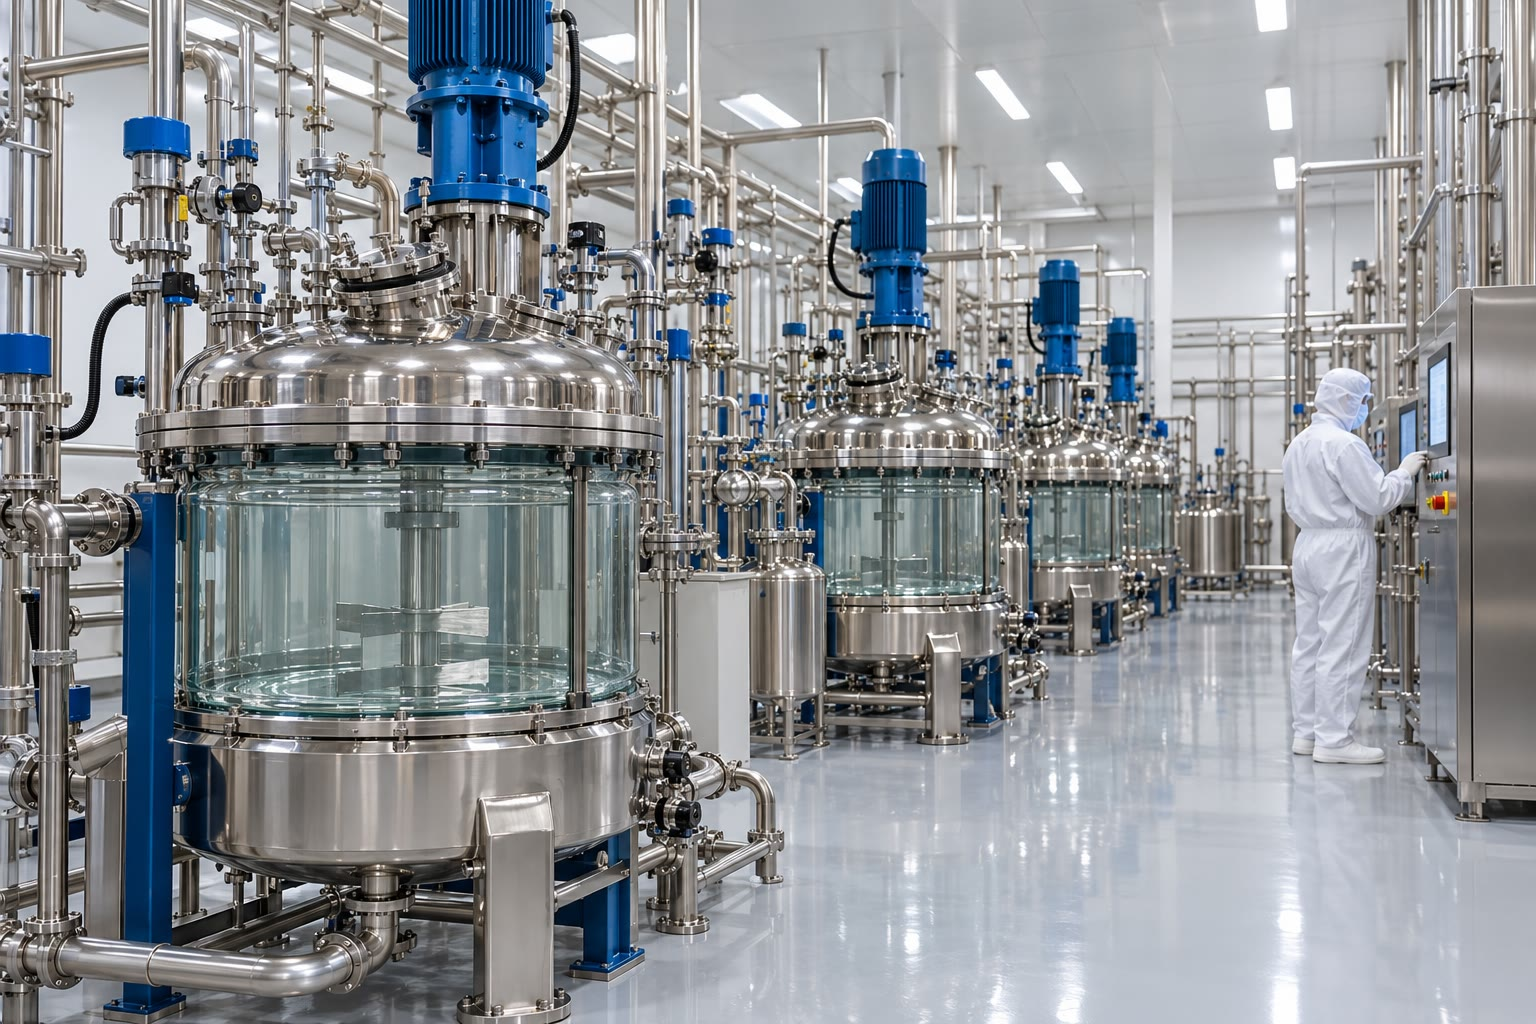
\includegraphics[width=0.58\linewidth]{images/book4/ai/b3-28-api-plant.jpg}

{\small A hall of glass-lined reactors in a plant making active
pharmaceutical ingredients. Many of its products are single enantiomers, made
by catalysis or resolution and checked by chiral chromatography.}
\end{omfigure}

\section{Measuring enantiopurity}

\begin{definition}[Enantiomeric excess]\label{def:b3:asymmetric-synthesis:ee}
For a mixture of enantiomers in amounts $n_R \ge n_S$, the \emph{enantiomeric
excess}\index{enantiomeric excess} is $\mathrm{ee} = (n_R - n_S)/(n_R + n_S)$ and the \emph{enantiomeric
ratio}\index{enantiomeric ratio} $\mathrm{er} = n_R/n_S$; for diastereomers, the
\emph{diastereomeric excess}\index{diastereomeric excess} de is defined in the
same way. The \emph{optical purity}\index{optical purity} is the ratio of the
specific rotation of a sample to that of the pure enantiomer.
\end{definition}

\begin{proposition}[ee and er]\label{prop:b3:asymmetric-synthesis:ee-er}
$\mathrm{ee} = (\mathrm{er} - 1)/(\mathrm{er} + 1)$ and $\mathrm{er} = (1 + \mathrm{ee})/(1 - \mathrm{ee})$.
\end{proposition}

\begin{proof}
Divide numerator and denominator of $(n_R - n_S)/(n_R + n_S)$ by $n_S$; solving for er gives the
second form.
\end{proof}

An ee of 90\,\% is an er of 95\,:\,5, an ee of 98\,\% an er of 99\,:\,1. \omterm{def:b3:asymmetric-synthesis:ee}{Optical purity}
equals ee only if rotation is proportional to composition; impurities, the
solvent, concentration effects and the small rotations of many compounds make
it unreliable, and ee is measured by separating the enantiomers.

\begin{method}[ee from a chiral chromatogram]\label{met:b3:asymmetric-synthesis:ee-chromatogram}
\begin{enumerate}
  \item Inject the racemate first, to identify the two peaks and check their
        separation (baseline resolution) and equal areas.
  \item Inject the sample and integrate both peaks.
  \item The enantiomers have the same response in an achiral detector, so
        $\mathrm{ee} = (A_1 - A_2)/(A_1 + A_2)$; assign the peaks with an enantiopure standard.
\end{enumerate}
\end{method}

\begin{omfigure}
\begin{tikzpicture}
\begin{axis}[name=a, width=0.48\linewidth, height=5.4cm, xmin=0, xmax=20, ymin=0, ymax=1.0,
  axis lines=left, xlabel={$\Delta\Delta G^\ddagger$ / \unit{kJ.mol^{-1}}}, ylabel={ee},
  tick label style={font=\scriptsize}, label style={font=\small}]
\addplot[omDef, thick] table[x=ddg, y=eeA] {figdata/out/bachelor-3-er-ddg.dat};
\addplot[omMeth, thick] table[x=ddg, y=eeB] {figdata/out/bachelor-3-er-ddg.dat};
\addplot[omThm, thick] table[x=ddg, y=eeC] {figdata/out/bachelor-3-er-ddg.dat};
\node[font=\scriptsize, omDef, anchor=west] at (axis cs:10,0.55) {\qty{-78}{\celsius}};
\node[font=\scriptsize, omMeth, anchor=west] at (axis cs:10,0.43) {\qty{0}{\celsius}};
\node[font=\scriptsize, omThm, anchor=west] at (axis cs:10,0.31) {\qty{25}{\celsius} (lowest curve)};
\end{axis}
\begin{axis}[at={(a.east)}, anchor=west, xshift=1.4cm, width=0.48\linewidth, height=5.4cm,
  xmin=7.5, xmax=9.5, ymin=0, axis lines=left, ytick=\empty,
  xlabel={retention time / min}, ylabel={detector signal},
  tick label style={font=\scriptsize}, label style={font=\small}]
\addplot[black, thick] table[x=t, y=y] {figdata/out/bachelor-3-er-ddg-b.dat};
\node[font=\scriptsize, anchor=south west] at (axis cs:8.3,250) {(\textit{R}): 97.5};
\node[font=\scriptsize, anchor=south] at (axis cs:9.1,20) {(\textit{S}): 2.5};
\end{axis}
\end{tikzpicture}

{\small Left: \omterm{def:b3:asymmetric-synthesis:ee}{enantiomeric excess} against the difference in \omterm{def:b3:rate-theories:activation}{Gibbs energy of
activation} of the two competing paths, at three temperatures: the same
$\Delta\Delta G^\ddagger$ gives a higher ee at low temperature. Right: a chiral HPLC chromatogram,
peak areas 97.5 and 2.5 (model): ee 95\,\%.}
\end{omfigure}

NMR distinguishes enantiomers only in a chiral environment: a chiral solvating
agent makes short-lived diastereomeric complexes whose signals differ, and a
chiral alcohol or amine converted into its two diastereomeric esters with
Mosher's acid shows the configuration from the pattern of shift differences.

\begin{method}[Configuration from Mosher esters, in outline]\label{met:b3:asymmetric-synthesis:mosher}
\begin{enumerate}
  \item Make both the (\textit{R})- and the (\textit{S})-MTPA esters of the alcohol.
  \item Record their proton spectra and compute $\Delta\delta = \delta_S - \delta_R$ for the protons on each
        side of the carbinol carbon.
  \item In the preferred conformation the phenyl ring of the acid shields one side:
        protons with $\Delta\delta > 0$ lie on one side, those with $\Delta\delta < 0$ on the other, which
        places the two substituents and gives the configuration.
\end{enumerate}
\end{method}

\section{Topicity and stereoselective additions}

\begin{definition}[Stereoselective reactions]\label{def:b3:asymmetric-synthesis:selective}
An \emph{enantioselective reaction}\index{enantioselective reaction} forms one
enantiomer of a product in excess over the other; a \emph{diastereoselective
reaction}\index{diastereoselective reaction} forms one diastereomer in excess.
\end{definition}

\begin{definition}[Topicity]\label{def:b3:asymmetric-synthesis:topicity}
Two groups of a molecule are \emph{homotopic}\index{homotopic} when exchanged by
a rotation of the molecule (replacing either gives the same compound),
\emph{enantiotopic}\index{enantiotopic} when exchanged only by a reflection
(replacing one or the other gives enantiomers), and
\emph{diastereotopic}\index{diastereotopic} when no \omterm{def:b3:point-groups:operation}{symmetry operation} exchanges
them (replacing one or the other gives diastereomers).
\end{definition}

The two hydrogens of a $\ce{CH2}$ group next to a stereocentre are \omterm{def:b3:asymmetric-synthesis:topicity}{diastereotopic}: they
have different chemical shifts and couple to each other, which is why such a
group often shows as two signals in NMR.

\begin{definition}[Prochiral faces]\label{def:b3:asymmetric-synthesis:faces}
A trigonal carbon with three different substituents is \emph{prochiral}\index{prochiral}:
addition of a fourth, different group creates a stereocentre. Its face seen with
the three substituents in decreasing CIP priority running clockwise is the
\emph{Re face}\index{Re face}; counterclockwise, the \emph{Si face}\index{Si face}.
\end{definition}

\begin{omfigure}
\begin{tikzpicture}[font=\small, >=Stealth]
  \coordinate (c) at (0,0);
  \draw[thick, double, double distance=1.6pt] (c) -- (90:1.1) node[above] {O (1)};
  \draw[thick] (c) -- (210:1.1) node[below left] {$\ce{C6H5}$ (2)};
  \draw[thick] (c) -- (330:1.1) node[below right] {$\ce{CH3}$ (3)};
  \fill (c) circle (1.6pt);
  \draw[->, thick, omThm] (70:0.6) arc[start angle=70, end angle=200, radius=0.6];
  \node[font=\scriptsize, omThm, align=center] at (-1.9,0.75) {1 $\to$ 2 $\to$ 3\\ counterclockwise:\\ \textit{Si} face};
  \node[font=\scriptsize, align=left, anchor=west] at (2.6,0.4) {face towards the reader: \textit{Si}\\ face behind the page: \textit{Re}};
  \node[font=\scriptsize, align=left, anchor=west] at (2.6,-0.5) {hydride added from the \textit{Re} face\\ gives (\textit{S})-1-phenylethanol};
\end{tikzpicture}

{\small The faces of acetophenone. Seen from the front, the substituents of the
carbonyl carbon in CIP order (O, phenyl, methyl) run counterclockwise: the front
face is \textit{Si}, the back face \textit{Re}.}
\end{omfigure}

\begin{method}[Assigning Re and Si faces]\label{met:b3:asymmetric-synthesis:re-si}
\begin{enumerate}
  \item Rank the three substituents of the trigonal atom by the CIP rules (a
        double bond counts its partner twice).
  \item Look at the face of interest, the trigonal plane in the plane of the page.
  \item Clockwise 1 $\to$ 2 $\to$ 3: \textit{Re}; counterclockwise: \textit{Si}.
  \item To name the product, add the new group towards the viewer and apply the
        CIP rules to the new stereocentre; Re attack does not always give \textit{R}.
\end{enumerate}
\end{method}

\begin{definition}[Felkin--Anh model and chelation control]\label{def:b3:asymmetric-synthesis:felkin}
The \emph{Felkin--Anh model}\index{Felkin--Anh model} predicts the major
diastereomer of a nucleophilic addition to a carbonyl group next to a
stereocentre: the largest group on that centre lies perpendicular to the
carbonyl plane, and the nucleophile approaches anti to it, past the smallest
group, along the Bürgi--Dunitz trajectory. Under \emph{chelation
control}\index{chelation control}, a metal ion bound to both the carbonyl oxygen
and a donor group on the stereocentre locks the conformation, and the
nucleophile adds to the less hindered face of the chelate ring.
\end{definition}

\begin{proposition}[Felkin--Anh selectivity]\label{prop:b3:asymmetric-synthesis:felkin}
For an $\alpha$-chiral aldehyde or ketone without a chelating group, the major
product is the one predicted by the \omterm{def:b3:asymmetric-synthesis:felkin}{Felkin--Anh model} (an empirical model,
supported by calculation). \admitted
\end{proposition}

\begin{omfigure}
\begin{tikzpicture}[font=\small, >=Stealth]
  \foreach \a/\lab in {90/L, 330/M, 210/S} {
    \draw[line width=0.8pt] (\a:0.55) -- (\a:1.1) node[pos=1.3] {\lab};
  }
  \fill[white] (0,0) circle (0.55);
  \draw[line width=0.8pt] (0,0) circle (0.55);
  \draw[line width=0.8pt, double, double distance=1.4pt] (0,0) -- (0:1.1) node[right] {O};
  \draw[line width=0.8pt] (0,0) -- (180:1.1) node[left] {R};
  \draw[->, very thick, omThm] (250:2.2) -- (250:0.25);
  \node[omThm, anchor=north] at (250:2.25) {Nu$^-$};
  \node[font=\scriptsize, align=left, anchor=west] at (1.7,-1.0) {Nu$^-$ enters anti to L,\\ past S, at about 107°\\ to the C=O bond};
\end{tikzpicture}

{\small \omterm{def:b3:asymmetric-synthesis:felkin}{Felkin--Anh model}, seen along the bond from the carbonyl carbon (front,
bonds to O and R) to the stereocentre (back circle, groups L, M and S). The
large group is perpendicular to the carbonyl plane; the nucleophile comes from
the opposite side, close to the small group and away from the oxygen.}
\end{omfigure}

\section{Strategies}

\begin{definition}[Chiral pool]\label{def:b3:asymmetric-synthesis:chiral-pool}
The \emph{chiral pool}\index{chiral pool} is the set of cheap, enantiopure
natural compounds (amino acids, sugars, terpenes, hydroxy acids) used as
starting materials, their stereocentres carried into the target.
\end{definition}

\begin{definition}[Chiral auxiliary]\label{def:b3:asymmetric-synthesis:auxiliary}
A \emph{chiral auxiliary}\index{chiral auxiliary} is an enantiopure group
attached temporarily to a substrate to control the stereochemistry of a
reaction, then removed and recovered.
\end{definition}

In Evans alkylations, an oxazolidinone made from an amino acid is acylated;
the lithium or sodium enolate, chelated to the auxiliary's carbonyl group, is
attacked by an alkyl halide on the face away from the auxiliary's substituent,
giving one diastereomer, often with de above 95\,\%; hydrolysis then frees the
chiral acid and the auxiliary.

\begin{definition}[Resolutions]\label{def:b3:asymmetric-synthesis:resolution}
The \emph{resolution of a racemate}\index{resolution of a racemate} is its
separation into enantiomers, classically by crystallising diastereomeric salts
with an enantiopure acid or base. In a \emph{kinetic resolution}\index{kinetic
resolution} the two enantiomers react at different rates with a chiral reagent or
catalyst, with selectivity $s = k_{\mathrm{fast}}/k_{\mathrm{slow}}$. In a \emph{dynamic kinetic
resolution}\index{dynamic kinetic resolution} the substrate enantiomers
interconvert fast while one of them reacts.
\end{definition}

\begin{theorem}[Kagan equation]\label{thm:b3:asymmetric-synthesis:kagan}
In a kinetic \omterm{def:b3:asymmetric-synthesis:resolution}{resolution of a racemate} by first-order reactions of selectivity $s$,
the conversion $c$ and the ee of the remaining substrate are related by
\[
  s = \frac{\ln[(1 - c)(1 - \mathrm{ee})]}{\ln[(1 - c)(1 + \mathrm{ee})]}.
\]
\end{theorem}

\begin{proof}
Each enantiomer decays exponentially: the fractions left are $f_1 = \eu^{-k_{\mathrm{fast}}t}$ and
$f_2 = \eu^{-k_{\mathrm{slow}}t}$, so $\ln f_1 = s\ln f_2$. Starting from equal amounts, $1 - c = (f_1 + f_2)/2$ and
$\mathrm{ee} = (f_2 - f_1)/(f_1 + f_2)$. Then $(1 - c)(1 - \mathrm{ee}) = \tfrac12(f_1 + f_2)\cdot 2f_1/(f_1 + f_2) = f_1$ and likewise
$(1 - c)(1 + \mathrm{ee}) = f_2$. Hence $s = \ln f_1/\ln f_2$ is the stated ratio.
\end{proof}

\begin{omfigure}
\begin{tikzpicture}
\begin{axis}[width=0.62\linewidth, height=5.6cm, xmin=0, xmax=1, ymin=0, ymax=1.02,
  axis lines=left, xlabel={conversion $c$}, ylabel={ee},
  tick label style={font=\scriptsize}, label style={font=\small},
  legend style={font=\scriptsize, draw=none, at={(1.04,0.5)}, anchor=west}, legend cell align=left]
\addplot[color=omThm, thick] table[x=c, y=eesm] {figdata/out/bachelor-3-kinetic-resolution-s2.dat};
\addlegendentry{$s = 2$}
\addplot[color=omMeth, thick] table[x=c, y=eesm] {figdata/out/bachelor-3-kinetic-resolution-s10.dat};
\addlegendentry{$s = 10$}
\addplot[color=omDef, thick] table[x=c, y=eesm] {figdata/out/bachelor-3-kinetic-resolution-s50.dat};
\addlegendentry{$s = 50$}
\addplot[color=omThm, thick, dashed] table[x=c, y=eep] {figdata/out/bachelor-3-kinetic-resolution-s2.dat};
\addplot[color=omMeth, thick, dashed] table[x=c, y=eep] {figdata/out/bachelor-3-kinetic-resolution-s10.dat};
\addplot[color=omDef, thick, dashed] table[x=c, y=eep] {figdata/out/bachelor-3-kinetic-resolution-s50.dat};
\end{axis}
\end{tikzpicture}

{\small \omterm{def:b3:asymmetric-synthesis:resolution}{Kinetic resolution}: ee of the remaining substrate (solid) and of the
product (dashed) against conversion, for three selectivities. The substrate
can always be made enantiopure by going far enough, at the cost of yield; the
product is purest at low conversion.}
\end{omfigure}

\begin{proposition}[Dynamic kinetic resolution]\label{prop:b3:asymmetric-synthesis:dkr}
If the substrate enantiomers interconvert much faster than either reacts, the
whole racemate can be converted into one product enantiomer, with ee set by $s$:
$\mathrm{er} = s$.
\end{proposition}

\begin{proof}
Fast racemisation keeps the two substrate enantiomers in equal amounts at all
times. The products then form at rates in the ratio $k_{\mathrm{fast}}[\mathrm A] : k_{\mathrm{slow}}[\mathrm A] = s$, and nothing
stops the reaction before all the substrate, through the fast enantiomer mostly,
is consumed: the yield can reach 100\,\% with $\mathrm{er} = s$.
\end{proof}

\begin{method}[Choosing a strategy]\label{met:b3:asymmetric-synthesis:strategy}
\begin{enumerate}
  \item If the target's stereocentres exist in a cheap natural compound, start
        from the \omterm{def:b3:asymmetric-synthesis:chiral-pool}{chiral pool}.
  \item For a one-off synthesis, or to set a centre reliably next to a carbonyl
        group, use an auxiliary, at the cost of two extra steps.
  \item If the racemate is cheap and the unwanted enantiomer can be recycled or
        racemised, resolve it (classically, kinetically or dynamically).
  \item For large scale, look for an asymmetric catalyst: one stereocentre made
        per catalytic turnover, no stoichiometric chiral waste.
\end{enumerate}
\end{method}

\section{Asymmetric catalysis with metals}

\begin{definition}[Asymmetric catalysis]\label{def:b3:asymmetric-synthesis:asymmetric-catalysis}
\emph{Asymmetric catalysis}\index{asymmetric catalysis} is enantioselective
synthesis with a chiral catalyst used in small amount; for metal catalysts, the
chirality usually comes from a \emph{chiral ligand}\index{chiral ligand}.
\end{definition}

\begin{theorem}[Selectivity from energy]\label{thm:b3:asymmetric-synthesis:er-ddg}
If two enantiomeric products are formed through diastereomeric transition states
with equal pre-exponential factors, irreversibly, under kinetic control,
$\mathrm{er} = \exp(\Delta\Delta G^\ddagger/RT)$, where $\Delta\Delta G^\ddagger$ is the difference of their Gibbs energies of
activation.
\end{theorem}

\begin{proof}
By the \omterm{thm:b3:rate-theories:eyring}{Eyring equation} (\cref{ch:b3:rate-theories}),
$k_i = (k_BT/h)\eu^{-\Delta G_i^\ddagger/RT}$; both products form from the same reactants, so at every moment
their rates are in the ratio $k_1/k_2 = \eu^{(\Delta G_2^\ddagger - \Delta G_1^\ddagger)/RT}$, and so are the amounts formed.
\end{proof}

At \qty{25}{\celsius} an ee of 99\,\% (er 199) needs $\Delta\Delta G^\ddagger = RT\ln 199 = \qty{13.1}{kJ/mol}$, about the energy of a
single hydrogen bond; at \qty{-78}{\celsius}, \qty{8.6}{kJ/mol} suffices.

\begin{proposition}[$C_2$-symmetric ligands]\label{prop:b3:asymmetric-synthesis:c2}
A $C_2$-symmetric \omterm{def:b3:asymmetric-synthesis:asymmetric-catalysis}{chiral ligand} halves the number of diastereomeric transition
states to be compared, since the two coordination sites it leaves are
equivalent.
\end{proposition}

\begin{proof}
The $C_2$ rotation of the catalyst maps one free site onto the other and leaves the
catalyst unchanged; any transition state at one site is therefore identical to
the rotated one at the other. Only the binding modes at one site (substrate face,
orientation) need to be compared.
\end{proof}

Knowles used chiral monophosphines, then the $C_2$-symmetric diphosphine DIPAMP, with rhodium to
hydrogenate an enamide to the protected amino acid of L-DOPA; Noyori's BINAP,
with ruthenium, hydrogenates ketones and functionalised alkenes, and,
combined with a chiral diamine, simple ketones with very high ee. In the
rhodium enamide hydrogenation the major product comes from the less stable,
minor catalyst--substrate complex, which reacts much faster with hydrogen: the
selectivity is set at the transition states, not by the \omterm{def:b3:partition-functions:boltzmann}{populations} of the
intermediates (the Curtin--Hammett principle).

\begin{definition}[Sharpless epoxidation]\label{def:b3:asymmetric-synthesis:sharpless}
The \emph{Sharpless epoxidation}\index{Sharpless epoxidation} is the
enantioselective epoxidation of allylic alcohols by \textit{tert}-butyl hydroperoxide,
catalysed by titanium(IV) isopropoxide with an enantiopure diethyl tartrate; the
alcohol binds to titanium, which delivers the oxygen to one face of the
alkene, chosen by the tartrate.
\end{definition}

\begin{omfigure}
\begin{tikzpicture}[font=\small, >=Stealth]
  \draw[black!50] (-2.3,-1.55) rectangle (2.5,1.55);
  % C3 (top) = C2 (bottom); C2 carries R1 (left) and CH2OH (lower right),
  % C3 carries R2 (left) and R3 (right)
  \coordinate (c3) at (0,0.45); \coordinate (c2) at (0,-0.45);
  \draw[thick, double, double distance=1.6pt] (c3) -- (c2);
  \draw[thick] (c3) -- (-0.9,0.95) node[above left, inner sep=1pt] {R$^2$};
  \draw[thick] (c3) -- (0.9,0.95) node[above right, inner sep=1pt] {R$^3$};
  \draw[thick] (c2) -- (-0.9,-0.95) node[below left, inner sep=1pt] {R$^1$};
  \draw[thick] (c2) -- (0.9,-0.95) node[below right, inner sep=1pt] {$\ce{CH2OH}$};
  \draw[->, very thick, omDef] (0.35,2.5) -- (0.2,0.1) node[pos=0, above, align=center, font=\scriptsize] {D-($-$)-diethyl tartrate:\\ O from the top face};
  \draw[->, very thick, omThm] (0.35,-2.6) -- (0.2,-0.1) node[pos=0, below, align=center, font=\scriptsize] {L-($+$)-diethyl tartrate:\\ O from the bottom face};
\end{tikzpicture}

{\small Sharpless's mnemonic. With the allylic alcohol drawn in the plane, the
$\ce{CH2OH}$ group at the lower right, L-($+$)-diethyl tartrate delivers the oxygen from
below the plane and D-($-$)-diethyl tartrate from above, whatever the
substituents $\mathrm R^1$ to $\mathrm R^3$.}
\end{omfigure}

The same idea, a metal held in a chiral pocket by a cheap natural ligand, gives
Sharpless's asymmetric dihydroxylation of alkenes with osmium and cinchona
alkaloid ligands. When the ligand is not enantiopure, the ee of the product
need not be proportional to that of the ligand: aggregates of two ligands, with
different activities for homochiral and heterochiral pairs, give non-linear
effects, sometimes useful amplifications.

\section{Organocatalysis}

\begin{definition}[Organocatalysis]\label{def:b3:asymmetric-synthesis:organocatalysis}
\emph{Organocatalysis}\index{organocatalysis} is catalysis by small organic
molecules without metals. In \emph{enamine catalysis}\index{enamine catalysis} a
secondary amine turns a ketone or aldehyde into a nucleophilic enamine; in
\emph{iminium catalysis}\index{iminium catalysis} it turns an $\alpha,\beta$-unsaturated
aldehyde into an electrophilic iminium ion with a lowered LUMO.
\end{definition}

\begin{omfigure}
\begin{tikzpicture}[font=\small]
  % proline-derived enamine and the aldehyde held by the carboxylic acid
  \coordinate (n) at (0,0.7); \coordinate (r2) at (0.67,0.22); \coordinate (r3) at (0.41,-0.57);
  \coordinate (r4) at (-0.41,-0.57); \coordinate (r5) at (-0.67,0.22);
  \draw[thick] (n) -- (r2) -- (r3) -- (r4) -- (r5) -- (n);
  \node[fill=white, inner sep=0.6pt] at (n) {N};
  \coordinate (ca) at (0,1.45); \coordinate (cb) at (0.72,1.85);
  \draw[thick] (0,0.88) -- (ca);
  \draw[thick] (ca) -- (-0.62,1.85) node[left, inner sep=1pt] {$\ce{CH3}$};
  \draw[thick, double, double distance=1.5pt] (ca) -- (cb);
  \coordinate (cacid) at (1.45,0.45);
  \draw[thick] (r2) -- (cacid);
  \draw[thick, double, double distance=1.5pt] (cacid) -- (1.75,-0.15) node[below, inner sep=1pt] {O};
  \draw[thick] (cacid) -- (2.05,0.9) node[right, inner sep=1pt] (oh) {O--H};
  \node (cald) at (1.55,2.55) {C};
  \draw[thick, double, double distance=1.5pt] (cald) -- (2.35,2.15) node[right, inner sep=1pt] (oald) {O};
  \draw[thick] (cald) -- (1.3,3.15) node[above, inner sep=1pt] {R};
  \draw[omThm, thick, densely dashed] (cb) -- (cald);
  \draw[omMeth, thick, dotted] (2.45,1.05) -- (2.5,2.0);
  \node[font=\scriptsize, omThm, anchor=east] at (1.05,2.35) {C--C forms};
  \node[font=\scriptsize, omMeth, anchor=west] at (2.6,1.55) {H bond};
\end{tikzpicture}

{\small The proline-catalysed aldol reaction, schematic transition state: the
enamine formed from acetone and the pyrrolidine nitrogen attacks the aldehyde,
whose oxygen is held by a hydrogen bond to the carboxylic acid of the catalyst;
that bond fixes which face of the aldehyde is attacked.}
\end{omfigure}

Proline, a cheap amino acid, catalyses intramolecular aldol reactions of
triketones with high ee (the Hajos--Parrish and Wieland--Miescher ketones, used
since the 1970s for steroid syntheses) and, as shown in 2000, intermolecular
aldol reactions of acetone with aldehydes. Chiral imidazolidinones work through
iminium ions in Diels--Alder reactions and conjugate additions; chiral
phosphoric acids, strong Brønsted acids with a chiral pocket, activate imines
by protonation. Organocatalysts are stable to air and water and leave no metal
in the product.

\begin{inthelab}[A chiral HPLC analysis]
A chiral column, silica coated with a cellulose or amylose derivative, is
equilibrated with a hexane--isopropanol mixture. The racemate is injected first
and the solvent ratio adjusted until the two peaks are baseline-separated; then
the sample, dissolved in the eluent at about a milligram per millilitre, is
injected, and the peaks integrated at a wavelength where both absorb.
\end{inthelab}

\begin{safety}{\ghs[0.6cm]{GHS02}\ghs[0.6cm]{GHS05}\ghs[0.6cm]{GHS06}\ghs[0.6cm]{GHS08}\ghs[0.6cm]{GHS09}}
% ledger: ghs4:TBHP, ghs4:TiOiPr4
\textit{tert}-Butyl hydroperoxide: flammable, self-reactive on heating, toxic in contact with
skin, corrosive, sensitising, suspected of causing genetic defects; it is used
as a solution, kept cool, never concentrated, and excess peroxide is destroyed
before work-up. Titanium(IV) isopropoxide: flammable, irritant, decomposed by
moisture.
\end{safety}

\begin{history}[Two prizes for asymmetric catalysis]
William Knowles, Ryoji Noyori and Barry Sharpless shared the 2001 Nobel Prize
in Chemistry for chirally catalysed hydrogenations and oxidations. Benjamin List
and David MacMillan, who had shown in 2000 that small organic molecules could
catalyse \omterm{def:b3:asymmetric-synthesis:selective}{enantioselective reactions} as broadly as metal complexes, received
the 2021 prize.
\end{history}

\section{Exercises}

\begin{exercise}[$\star$]\label{exo:b3:asymmetric-synthesis:1}
Convert: ee 80\,\% to er; er 99\,:\,1 to ee; ee 50\,\% to the percentage of each
enantiomer.
\end{exercise}

\begin{exercise}[$\star$]\label{exo:b3:asymmetric-synthesis:2}
A chiral HPLC trace shows peaks of areas 1840 and 60 for the two enantiomers.
Compute the ee.
\end{exercise}

\begin{exercise}[$\star$]\label{exo:b3:asymmetric-synthesis:3}
Assign the Re and \omterm{def:b3:asymmetric-synthesis:faces}{Si faces} of propanal's carbonyl carbon, and name the alcohol
formed by addition of a methyl nucleophile to the \omterm{def:b3:asymmetric-synthesis:faces}{Re face}.
\end{exercise}

\begin{exercise}[$\star$]\label{exo:b3:asymmetric-synthesis:4}
Are the two methylene protons of ethanol \omterm{def:b3:asymmetric-synthesis:topicity}{homotopic}, \omterm{def:b3:asymmetric-synthesis:topicity}{enantiotopic} or \omterm{def:b3:asymmetric-synthesis:topicity}{diastereotopic}?
And those of the $\ce{CH2}$ group of 2-butanol?
\end{exercise}

\begin{exercise}[$\star\star$]\label{exo:b3:asymmetric-synthesis:5}
Compute the $\Delta\Delta G^\ddagger$ needed for 99\,\% ee at \qty{25}{\celsius} and at \qty{-78}{\celsius}, and the ee given at \qty{-78}{\celsius}
by a catalyst that gives 80\,\% ee at \qty{25}{\celsius} (same $\Delta\Delta G^\ddagger$).
\end{exercise}

\begin{exercise}[$\star\star$]\label{exo:b3:asymmetric-synthesis:6}
A sample of an amine has $[\alpha]_D = -12.0$ under conditions where the pure (\textit{S})
enantiomer has $-15.0$ (data of the exercise). Give its \omterm{def:b3:asymmetric-synthesis:ee}{optical purity} and the
percentages of the enantiomers, assuming rotation proportional to composition.
Why is this measurement less reliable than chromatography?
\end{exercise}

\begin{exercise}[$\star\star$]\label{exo:b3:asymmetric-synthesis:7}
In a lipase-catalysed acetylation of a racemic alcohol, the remaining alcohol
has 90\,\% ee at 60\,\% conversion. Compute $s$.
\end{exercise}

\begin{exercise}[$\star\star$]\label{exo:b3:asymmetric-synthesis:8}
Predict the epoxide formed from (\textit{E})-hex-2-en-1-ol with L-($+$)-diethyl tartrate, and with
D-($-$)-diethyl tartrate.
\end{exercise}

\begin{exercise}[$\star\star$]\label{exo:b3:asymmetric-synthesis:9}
(\textit{S})-2-phenylpropanal is treated with methylmagnesium bromide. Use the \omterm{def:b3:asymmetric-synthesis:felkin}{Felkin--Anh
model} to predict the major diastereomer.
\end{exercise}

\begin{exercise}[$\star\star\star$]\label{exo:b3:asymmetric-synthesis:10}
Show that in a \omterm{def:b3:asymmetric-synthesis:resolution}{kinetic resolution} the product ee tends to $(s - 1)/(s + 1)$ at low
conversion, and compute it for $s = 20$. Why is a \omterm{def:b3:asymmetric-synthesis:resolution}{kinetic resolution} better at purifying
the substrate than at making the product?
\end{exercise}

\begin{exercise}[$\star\star\star$]\label{exo:b3:asymmetric-synthesis:11}
A ketone with a racemisable stereocentre next to the carbonyl group is reduced by
an \omterm{def:b3:complex-kinetics:enzyme}{enzyme} with $s = 99$, while racemisation is fast. What yield and ee can be
reached? Compare with the same \omterm{def:b3:complex-kinetics:enzyme}{enzyme} without racemisation, stopped at 50\,\%
conversion.
\end{exercise}

\begin{exercise}[$\star\star\star$]\label{exo:b3:asymmetric-synthesis:12}
Explain with the Curtin--Hammett principle how the minor catalyst--substrate
complex can give the major product, using two complexes in equilibrium
($K = 10$ in favour of A) that react with $k_B/k_A = 600$.
\end{exercise}

\section{Problem: The L-DOPA Route}

\begin{problem}[{Weekend problem --- the L-DOPA route: the prochiral enamide and its
faces, the energy behind 95\,\% ee, purification by crystallisation, and what a
kinetic resolution would have needed}]
\label{pb:b3:asymmetric-synthesis:1}
% ledger: const:R
Data of the problem: the rhodium-catalysed hydrogenation of the enamide
precursor at \qty{25}{\celsius} gives the protected (\textit{S})-amino acid with 95\,\% ee. The crude
product, 100 g, is recrystallised: the mother liquor retains all of the minor
enantiomer and 5.0 g of the major one.

\medskip\noindent\textbf{Part I --- The substrate.}
\begin{enumerate}
  \item Why is the enamide \omterm{def:b3:asymmetric-synthesis:faces}{prochiral}? Which carbon becomes a stereocentre?
  \item What would an achiral catalyst give?
  \item Why does the amide group on the alkene matter for the catalyst?
  \item What does the chiral diphosphine do?
  \item Is the major product formed from the more stable catalyst--substrate
        complex?
  \item Why is hydrogen added to one face only in each complex?
\end{enumerate}

\medskip\noindent\textbf{Part II --- Energy.}
\begin{enumerate}[resume]
  \item Give the er for 95\,\% ee.
  \item Compute $\Delta\Delta G^\ddagger$ at \qty{25}{\celsius}.
  \item What ee would the same $\Delta\Delta G^\ddagger$ give at \qty{-78}{\celsius}?
  \item What ee would a $\Delta\Delta G^\ddagger$ larger by \qty{2}{kJ/mol} give at \qty{25}{\celsius}?
  \item Compare \qty{9}{kJ/mol} with the energy of a hydrogen bond, and comment.
  \item Why is the reaction not simply run colder?
\end{enumerate}

\medskip\noindent\textbf{Part III --- Crystallisation.}
\begin{enumerate}[resume]
  \item Compute the masses of the two enantiomers in the crude product.
  \item Compute the mass and ee of the crystals.
  \item Compute the yield of the crystallisation.
  \item Why can crystallisation raise the ee of a sample but never create it from a
        racemate (for a compound that crystallises as a racemic compound)?
  \item How is the final ee checked?
\end{enumerate}

\medskip\noindent\textbf{Part IV --- A \omterm{def:b3:asymmetric-synthesis:resolution}{kinetic resolution} instead.}
\begin{enumerate}[resume]
  \item What is the maximum yield of one enantiomer by a simple \omterm{def:b3:asymmetric-synthesis:resolution}{kinetic resolution}?
  \item Compute the $s$ needed for 95\,\% ee of the remaining substrate at 55\,\% conversion.
  \item What yield of that substrate is obtained?
  \item How would a \omterm{def:b3:asymmetric-synthesis:resolution}{dynamic kinetic resolution} change the yield?
  \item Why was asymmetric hydrogenation the better industrial choice?
  \item Why must the rhodium be removed from the drug, and how is it measured?
  \item State the result: the $\Delta\Delta G^\ddagger$ for 95\,\% ee at \qty{25}{\celsius}.
\end{enumerate}
\end{problem}
